% VDE Template for EUSAR Papers
% Provided by Barbara Lang und Siegmar Lampe
% University of Bremen, January 2002
% English version by Jens Fischer
% German Aerospace Center (DLR), December 2005
% Additional modifications by Matthias Wei{\ss}
% FGAN, January 2009

%-----------------------------------------------------------------------------
% Type of publication
\documentclass[a4paper,10pt]{article}
%-----------------------------------------------------------------------------
% Other packets: Most packets may be downloaded from www.dante.de and
% "tcilatex.tex" can be found at (December 2005):
% http://www.mackichan.com/techtalk/v30/UsingFloat.htm
% Not all packets are necessarily needed:
\usepackage[T1]{fontenc}
\usepackage[latin1]{inputenc}
%\usepackage{ngerman} % in german language if required
\usepackage[nooneline,bf]{caption} % Figure descriptions from left margin
\usepackage{times}
\usepackage{multicol}
\usepackage{amsmath}
\usepackage{amssymb}
\usepackage[dvips]{graphicx}
\usepackage{epsfig}
\input{tcilatex}
%-----------------------------------------------------------------------------
% Page Setup
\textheight24cm \textwidth17cm \columnsep6mm
\oddsidemargin-5mm                 % depending on print drivers!
\evensidemargin-5mm                % required margin size: 2cm
\headheight0cm \headsep0cm \topmargin0cm \parindent0cm
\pagestyle{empty}                  % delete footer and header
%----------------------------------------------------------------------------
% Environment definitions
\newenvironment*{mytitle}{\begin{LARGE}\bf}{\end{LARGE}\\}%
\newenvironment*{mysubtitle}{\bf}{\\[1.5ex]}%
\newenvironment*{myabstract}{\begin{Large}\bf}{\end{Large}\\[2.5ex]}%
%-----------------------------------------------------------------------------
% Using Pictures and tables:
% - Instead "table" write "tablehere" without parameters
% - Instead "figure" write "figurehere " without parameters
% - Please insert a blank line before and after \begin{figuerhere} ... \end{figurehere}
%
% CAUTION:   The first reference to a figure/table in the text should be formatted fat.
%
\makeatletter
\newenvironment{tablehere}{\def\@captype{table}}{}
\newenvironment{figurehere}{\def\@captype{figure}\vspace{2ex}}{\vspace{2ex}}
\makeatother



%%%%%%%%%%%%%%%%%%%%%%%%%%%%%%%%%%%%%%%%%%%%%%%%%%%%%%%%%%%%%%%%%%%%%%%%%%%%%%
\begin{document}

% Please use capital letters in the beginning of important words as for example
\begin{mytitle}Internet of Things\end{mytitle}
\begin{mysubtitle}Focus on Contiki, a RTOS design for IoT\end{mysubtitle}
%
% Please do not insert a line here
%
\\
Allevi Daniele\\
Matr. 798891, (daniele.allevi@polimi.it)\\
\hspace{10ex}
\begin{flushright}
\emph{Report for the master course of Real time operating system}\\
\emph{Reviser: PhD. Patrick Bellasi (bellasi@elet.polimi.it)}
\end{flushright}

Received: November, 11 2013\\
\hspace{10ex}

\begin{myabstract} Abstract \end{myabstract}
Internet of things is a very hot topic in recent years, particularly with the massive spread of smart devices always connection to the network. Moreover the concept of internet of things can be used for multiple fields from simply monitoring  environment to a more complex project like smart city, where the information that sensor capture can be used to make decision and give order to actuators. Other examples are continuous care, emergency response, intelligent shopping, smart product management, smart meters, home automation and smart events.

 Future systems will be ever more complex that now with the increase of the methods of connection between objects. Almost every electric object will contain an embedded system that will be communicate with the other system and take decision on the base to the information that will receive from others. This report has the aim to explain the main ideas on internet of things, examining one of the real time operating system developed for internet of things: Contiki.


\vspace{4ex}	% Please do not remove or reduce this space here.
\begin{multicols}{2}

%%%%%%%%%%%%%%%%%%%%%%%%%%%%%%%%%%%%%%%%%%%%%%%%%%%%%%%%%%%%%%%%%%%%%%%%%%%%%
\section{Introduction to Internet of Things}

Internet of things is a concept and a paradigm that considers pervasive presence in the environment of a variety of things/objects that through wireless and wired connections are able to interact with each other and cooperate with other things/objects to create new application/service and reach common goals. \cite{Ovidiu13Internet}  




%-----------------------------------------------------------------------------
\subsection{Characteristics of IoT}
% Please avoid separations in titles
% and separate text manually

 A fundamental characteristic of IoT is to map things between
 physical world and cyber world. Physical world include physical
 things, or else, something that is possible to detect easily with
 human sense like object, behaviors, physical event. From the 
other side, cyber world include cyber things, or else,  something
 that is possible to elaborate and share with the ICT like entities,
 cyber actions (data transmission), cyber events (online payment), 
services (Email). (see {\bf Figure\ref{fig:myfigure1}})\\


We can distinguish three main features of IoT:\\\\
-Capability of perceive: try to imitate the sense of human
 (vision, hearing, smell and touch) in order to realize the intrinsic 
computation that humans do every day, that is things identification.\\\\
- Network of networks: try to connect many kinds of networks, from 
access networks in the sensor-actuator layer up to the heterogeneous 
communication of the many node such as cable communication, mobile 
communication (GSM, LTE),  wireless communication.\\\\
- Intelligent processing:  the capability needed to process and manage 
all the amount of information that the sensors perceive and to send the
 commands to the actuators in order to respond in the right way in
 every situation. In particular we want that the IoT will able to
 perform learning from the past, with the huge amount of information 
that the system has stored in the time.


\begin{figurehere}
 \centering
 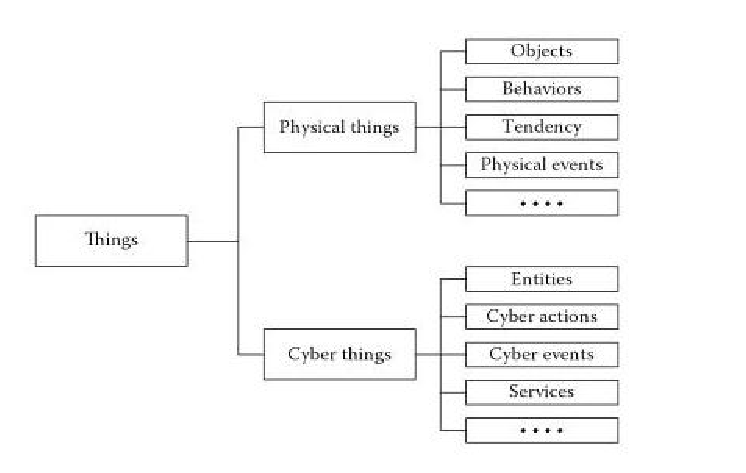
\includegraphics[width=10cm, height=6cm]{./eps/Things.eps}
 \caption{The classification of physical and cyber things in the Internet of Things}
 \label{fig:myfigure1}
\end{figurehere}

%-----------------------------------------------------------------------------


\subsection{Technology integration}

An important aspect is that the information is retrieved from many sensors, each with a potentially different technology, so is necessary that the software and hardware are based on the integration of information technology.\\ For example the software needs to take into account that there are a very large number of highly heterogeneous data sources, with different data structuring levels. All this factors require to the software to combine data coming from different data sources, providing a unified vision of the data necessary to elaborate it.\\The rapid convergence of information and communications technology is taking place at three layers of technology innovation:\\\\
- The cloud: Place where to find information, internet service, broadcast services, telecommunication value-added services.\\\\
- Communication networks: transmission medium where information travels, traditional communication networks, internet data communication networks, cable networks.\\\\
- Device: terminal level includes personal electronic device, telecommunication, but also sensor to retrieve information.


%-----------------------------------------------------------------------------
\subsection{Barriers}
IoT will face many hurdles, including security, privacy, and reliability, while other problems will require us to have open social and political discussions. In addition to these challenges, many technical barriers will need to be overcome 
as IoT pushes the boundaries of what we know is possible today with regard to 
network protocols, storage, and analytics. For example, IPv6 must become a reality 
as the number of connections moves from billions to trillions. Other challenges 
include finding energy sources for powering the huge number of miniature (even 
microscopic) devices.\\

Since that we have a network of nodes that contain sensitive information , security is an aspect to take into account. 
We can distinguish two categories of devices:\\\\
-Critical Infrastructure, like power production and distribution, manufacturing, transportation\\\\
- Personal infrastructure, like personal medical devices, automobiles, home entertainment and device control.\\\\
In the first case the major risk could be the interruption of primary services, for example furniture of water or electricity. In the second case, the risks are about privacy and health.\\

These few examples are sufficient to understand that a security problem inside a network can cause catastrophic effect, so new technology are required to protect all types of network connection that we have, considering that we have not only a "big" devices like laptop but the major devices in these networks are embedded system.
In the embedded system usually security is not taken into account because a lot of these products are cheap and there is a lot of competition, so it's usually not a good security architecture designs.

\begin{figurehere}
 \centering
 \includegraphics[width=9cm, height=6cm]{./eps/Ioe.eps}
 \caption{Internet Growth}
 \label{fig:myfigure2}
\end{figurehere}

%-----------------------------------------------------------------------------
\subsection{Conclusion}


What’s revolutionary in all this is that these physical information systems are now 
beginning to be deployed, and some of them even work largely without human intervention.\\
\cite{cisco12}  From Cisco's point of view, now we are in a transition era, where many
 organizations are currently experiencing the Internet of Things and tomorrow will arrive
 the Internet of Everything(IoE)  (see {\bf Figure\ref{fig:myfigure2}}).
A term used by Cisco to mark the fact that IoT becomes a network of networks where
 billions or even trillions of connections create unprecedented opportunities as well as
 new risks.\\ This can be explained by the exponential power of networks, commonly
 referred to as network effects often it associated with Metcalfe’s law.\\
 Metcalfe's law states that the value of a telecommunications network is proportional 
to the square of the number of connected users of the system. In easy words, a network
 effect is generated when participants, or nodes within a network are connected in a
 manner makes the whole greater than the sum of its parts.\\ By combining people,
 process, data, and things, the exponential power of the Internet will allow to create
 exponential responses to the extraordinary challenges faced by individuals(People
 experience the world through their senses), businesses(optimization and efficiencies),
 and countries(increase the level of transparency).




%%%%%%%%%%%%%%%%%%%%%%%%%%%%%%%%%%%%%%%%%%%%%%%%%%%%%%%%%%%%%%%%%%%%%%%%%%%%%
\section{Contiki}

\cite{wiki} Contiki is an open source operating system for networked, 
memory-constrained systems with a particular focus on low-power wireless
 Internet of Things devices.\\ Examples of where Contiki is used include street
 lighting systems, sound monitoring for smart cities, radiation monitoring systems,
 and alarm systems

%-----------------------------------------------------------------------------
\begin{figurehere}
 \centering
 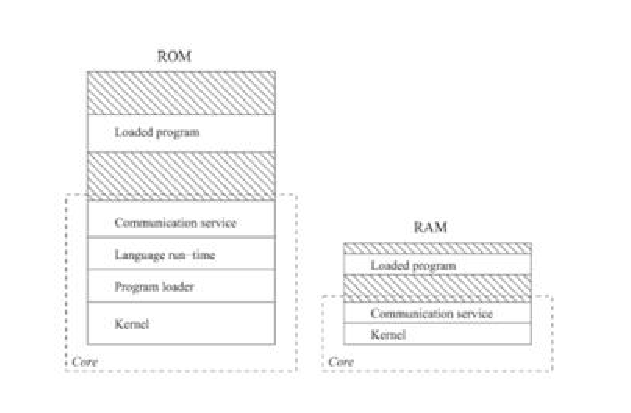
\includegraphics[width=9cm, height=6cm]{./eps/system.eps}
 \caption{Contiki system architecture}
 \label{fig:myfigure3}
\end{figurehere}


\subsection{System architecture}
A Contiki system is partitioned into two parts: the core and the loaded programs. 
The partitioning is made at compile time and it is specific to the deployment in which Contiki is used.
The core contains the Contiki kernel, the program loader, that places programs into
 memory and prepares them for execution, run-time and support libraries, and a
 communication stack with device drivers for the communicaton hardware.
The core is compiled into a single binary image that is stored in the devices prior to
 deployment. The core is generally not modified after deployment, even though it is 
possible to use a special boot loader to overwrite or patch the core (see {\bf Figure \ref{fig:myfigure3}}).


\begin{figurehere}
 \centering
 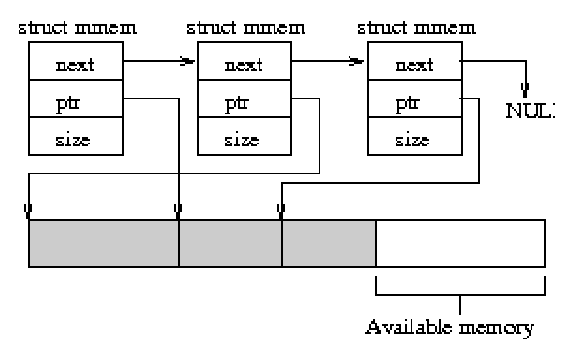
\includegraphics[width=8cm, height=6cm]{./eps/mmem.eps}
 \caption{Managed memory allocator}
 \label{fig:myMmem}
\end{figurehere}

 

%-----------------------------------------------------------------------------
\subsection{Memory allocation}

Contiki provides three possibility of \cite{support} memory allocation:\\\\
- Memory block allocator: permit to operate with a set of memory blocks of fixed size.
 Every set  is statically declared with an array. This is a flexible solution because the
 programmer can manage completely the memory allocation, but more complex. 
This is the most common solution used in Contiki.\\\\
- Managed memory allocator: provides a dynamic memory allocation with functions
 like malloc in C, that allows to ask for a specific amount of memory using a list for data structure.
The difference from the normal C malloc is that when the free function is called 
for a specific block, the system compacts the remaining memory, in the specific 
all memory following the deallocated block is moved downwards to start at the newly 
freed position, keeping the allocated memory free from fragmentation (see {\bf Figure \ref{fig:myMmem}}).
This solution is easiest because system is responsible to manage the memory,
 but less flexible. In particular is unsafe to use in preemptible code if it is also used
 in interrupt handlers or in multi threading. A module that uses a memory block could 
find its memory block relocated if the preemptive code called free. 
Normally this method is used only within Contiki processes. Although such processes are 
cooperatively scheduled, it is necessary to ensure that each pointer to an address
 within in the memory block is updated when the process resumes control after waiting for an event.\\\\
- The malloc Heap Memory Allocator: the usually functions used in C



%-----------------------------------------------------------------------------
\begin{figure*}[t]
  \centering
 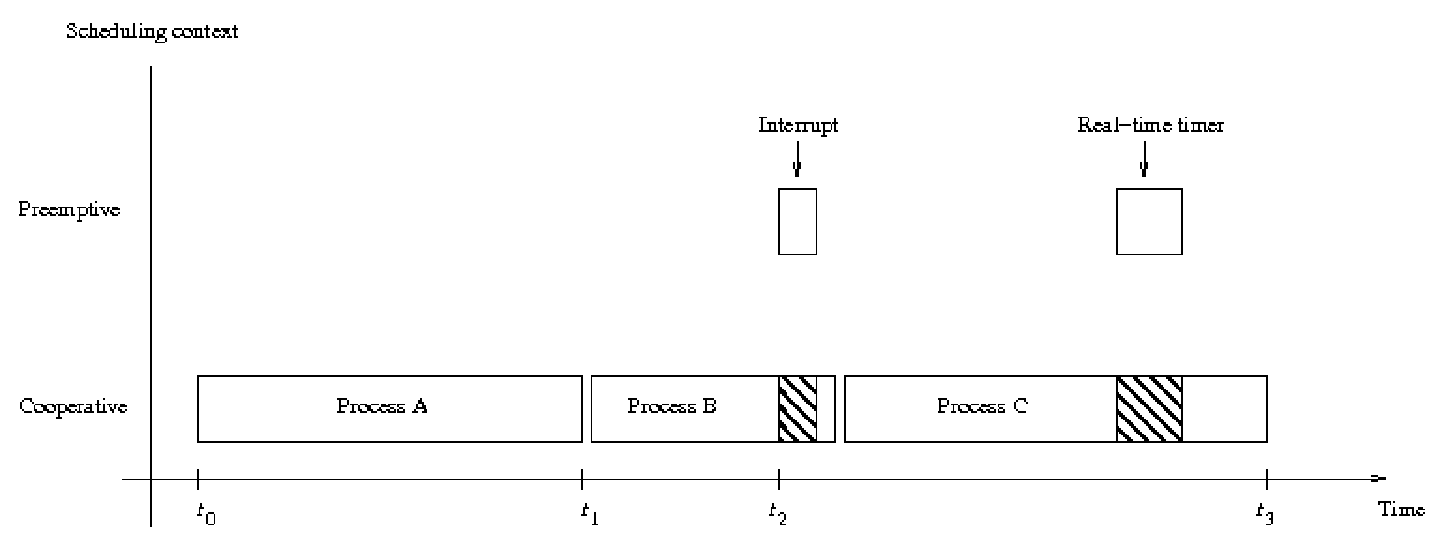
\includegraphics[width=10cm, height=4cm]{./eps/execution_contexts.eps}
\caption{Exection contexts}
 \label{fig:myfigure4}
\end{figure*}
\subsection{Scheduling}

Contiki provides two execution mode: cooperative or preemptive. Cooperative code runs sequentially with respect to other cooperative and must finish before other cooperatively scheduled code can run. Preemptive code may stop the cooperative code at any time. When preemptive code stops the cooperative code, the cooperative code will not be resumed until the preemptive code has completed.
Normal processes run in the cooperative context, whereas interrupts and real-time timers run in the preemptive context.(see {\bf Figure \ref{fig:myfigure4}})\\
A process consists of two parts: a process control block(PCB) and a process thread. The PCB, which is stored in RAM, contains run-time information about the processes, is lightweight: it requires only a couple of bytes of memory. The process thread is the code of the process, is stored in ROM and is a single protothread (we will see it in the section 3) that is invoked from the process schedule. 
In Contiki, a process is run when it receives an event, asynchronous or synchronous . There is a kernel's event queue where processes posts asynchronous events for delivering later to the destination process. The kernel loops through the event queue and delivers the events to the processes on the queue by invoking the processes. In case of post asynchronous event, it is immediately delivered to the receiving process.
There is also a special type of event: poll request, that causes the process to be scheduled as quickly as possible.
Polling is the way to make a process run from an interrupt.\\ 
 All process invocation is done in response to an event being posted to a process, or a poll has being requested for the process, the process scheduler passes the event identifier to the process that is being invoked. With the event identifier, an opaque pointer is passed. The pointer is provided by the caller and may be set to NULL to indicate that no data is to be passed with the event.\\
Processes have two possibility to terminate, by itself exits, or it is killed by another process.
When a process terminate, the Contiki kernel send an event to all other processes to inform them. This can be used by other processes to free up any resource allocations made by the process that is exiting. For example, the micro IP TCP/IP stack will close and remove any active network connections that the exiting process has.


%-----------------------------------------------------------------------------
\subsection{Coffee flash file system}

In the world of the embedded systems, in particular for the nodes that are used for sensors,
 devices needs to have an an external flash memory chip, in order to store the information that capture from the environment.\\ To manage this memory easily, Contiki provides a lightweight flash file system, called Coffee.
With Coffee, application programs can open, close, read from, write to, and append to files on
 the external flash, without having to worry about flash sectors needing to be erased before
 writing or flash wear-leveling.\\Coffee uses sequential page structures for files. The sequential 
structure can be reserved with a certain size. If a file has not been reserved when it is opened for
 the first time, it will be allocated with a default size.\\ When the user want to delete a something,
 the file system will not erase physically the file from the storage device, but only mark it as obsolete,
 this happens to speed up the process to remove a file. The physically remove will happen in a second time,
 that is when new file reservation request cannot be granted. The garbage manage this operation,
 in particular search sequentially over the storage device, which is divided into an array of sectors.
 For each sector it checks if the sector contains at least one obsolete page and no active pages. If 
the check succeeds, Coffee erases the sector. There is a possibility that obsolete pages spans more 
sectors than the one being erased, but in that case Coffee splits the remaining pages into isolated pages
 that belong to no file. The isolated pages are treated in the same way as obsolete pages when they are processed by the garbage collector.\\ The most essential part of Coffee is the quick-skip algorithm for finding file
 extents. The file allocation rules enables this algorithm to quickly jump over free areas and 
allocated extents after reading single headers and determining their status. The worst-case 
performance occurs when we encounter multiple long sequences of isolated pages, but such
 sequences are uncommon and always shorter than a sector.
The performance of Coffee is within 95\% \cite{site} of the raw throughput of the flash memory.




%%%%%%%%%%%%%%%%%%%%%%%%%%%%%%%%%%%%%%%%%%%%%%%%%%%%%%%%%%%%%%%%%%%%%%%%%%%%%
\section{Contiki for IoT}

In this section it will list the main features that make Contiki a good operating system for the IoT.


%-----------------------------------------------------------------------------
\subsection{Dynamic reprogramming}

In the internet of thing, the situation to update the software of the sensor is common, but this operation need to be execute without turn off the system and it is unthinkable to update physically one by one the sensors so the possibility to loading and linking modules at run time, it's extremely important.\\
Contiki supports this features, can load individual program from the network, which makes it possible to dynamically reprogram the behavior of the network. There are two possibility:\\\\
- Using the Executable Linkable Format (ELF): An ELF file consists of a header followed by a set of sections which typically include at least a section for binary code (.text), a section for statically allocated data with pre-assigned values (.data), and a section for zero-initialized data(.bss). Additionally, each symbol is represented in a symbol table, and strings are stored in a string table. Contiki can load either a freestanding program or a code module. The dynamic loader links, relocates ELF objects files into the Contiki system image.\\\\

- Using the native executable format: Contiki includes a module that can load software. It needs an argument consist of an opaque pointer to data that will be supplied as an argument to the process located in the loaded module as soon as it is started.
Unlike the ELF loader implementation, now the system automatically starts processes that have been defined in auto start processes variable of the loaded module. The consequence of this is that such modules must have the auto start processes variable defined.

\begin{figurehere}
 \centering
 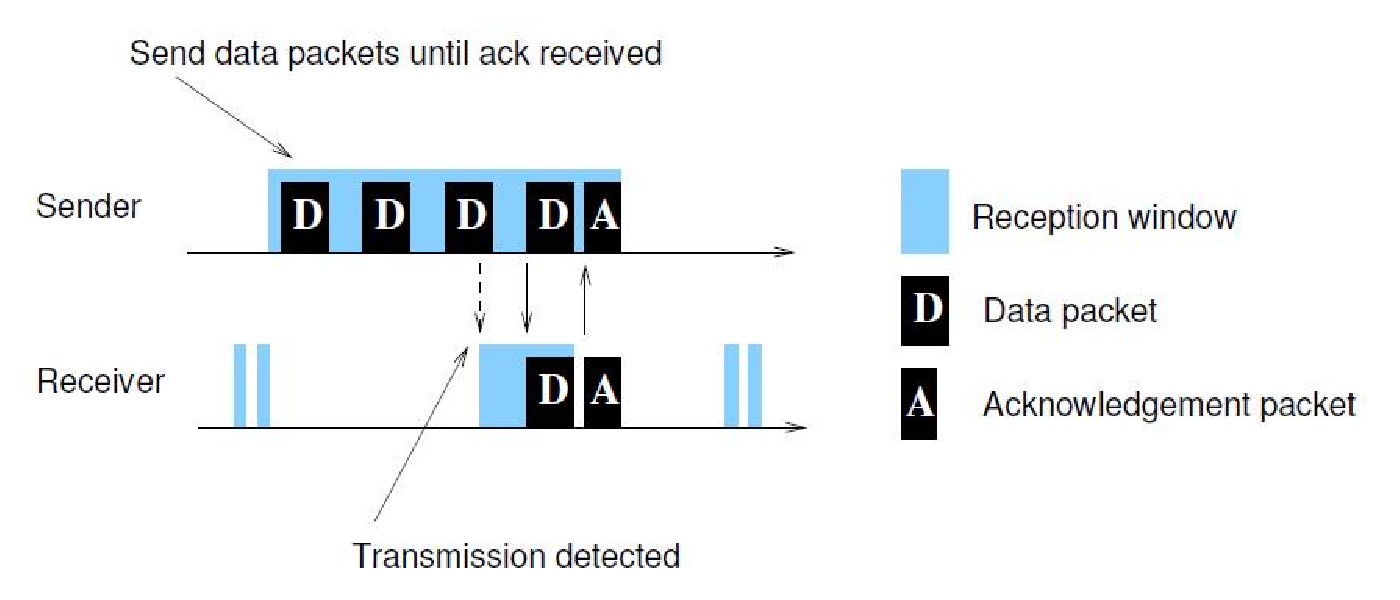
\includegraphics[width=8cm, height=6cm]{./eps/ContikiMAC.eps}
 \caption{Contiki MAC transission}
 \label{fig:myMAC}
\end{figurehere}


%-----------------------------------------------------------------------------
\subsection{Energy Saving}

\subsubsection{Power Awareness}
The major part of the devices that uses Contiki are systems that may need to work for years with a very small battery, so it's not thinkable to  change battery hundreds or thousand of times every six months. It's necessary a mechanism that can estimate the power consuption of the all components of the device, in order to develop a code that providing a lower energy consumption.
In particular Contiki has a class: energest that provides all type of component that you want to estimate the power consumption, like CPU, flash read/write etc. There's also a function(energest type time) that take a parameter that indicate the component that you want to estimate and returns its time of run. So, if you want to estimate the power consuption, it's necessary to call it a first time before start to work, and another time in a loop, and calculate the difference between the two return values to obtain the time of run. Done this we can calculate the power consuption multiplying the time of run with the values of current and voltage(taken from datasheet), divided by 4096 number of ticks per second.



\subsubsection{Radio Duty Cycling Protocol}

As introduced before in IoT, a fundamental aspect is the phase to take information from the environment, and to do this we saw that we need a very large network of sensor that can distribute information between nodes, so it's necessary to put some nodes that behave like a router, receive and routes messages from nodes to their destination.
These operations are extremely expensive from the point of view of power consumption, so the challenge is to keep the radio transceivers off as much as possible to reach a low power consumption, and at the same time must wake up often enough to be able to receive communication from their neighbors.
To do this, Contiki provides a mechanism called ContikiMAC radio duty cycling, that ensure nodes can participate
in network communication yet keep their radios turned off for roughly 99% of the time.
The mechanism is based on the concept that the wireless transceiver consumes as much power when passively listening for transmission from other devices respect to when actively transimitting, so transceiver must be completely turned off to save power.
ContikiMAC uses periodical wake-ups to listen for packet transmissions from neighbors. If a packet transmission is detected during a wake-up, the receiver is kept on to be able to receive the packet. When the packet is successfully received, the receiver sends a link layer acknowledgment. To transmit a packet, a sender repeatedly sends its packet until it receives a link layer acknowledgment from the receiver. Packets that are sent a broadcasts do not result in linklayer acknowledgments. Instead, the sender repeatedly sends the packet during the full wake-up interval to ensure that all neighbors have received it (see {\bf Figure \ref{fig:myMAC}}).


%-----------------------------------------------------------------------------
\subsection{Timers}

As in any other real time operating systems, timers are fundamental, especially for respect the deadlines. In the IoT systems, the same speech is true, but also remembering the constraints of energy, they can be used by applications to enter low power mode for a time period before resuming execution.


Contiki has one clock module and a set of timer modules: timer, stimer, ctimer, etimer, and rtimer. 
The clock module provides two functions for blocking the CPU: CLOCK DELAY() which blocks the CPU for a specified delay, and CLOCK WAIT(), which blocks the CPU for a specified number of clock ticks. These functions are normally only used in low-level drivers where it sometimes is necessary to wait a short time without giving up the control over the CPU.
While the different timer modules \cite{support} have different uses:\\\\ 
- The timer and stimer libraries provides the simplest form of timers and are used to check if a time period has passed. The applications need to ask the timers if they have expired. The difference between these is the resolution of time: timers use system clock ticks while stimers use seconds to allow much longer time periods. Unlike the other timers, the timer and stimer libraries can be safely used from interrupts which makes them especially useful in low level drivers.\\\\
- The etimer library provides event timers and are used to schedule events to Contiki processes after a period of time. They are used in Contiki processes to wait for a time period while the rest of the system can work or enter low power mode.\\\\
- The ctimer library provides callback timers and are used to schedule calls to callback functions after a period of time. Like event timers, they are used to wait for some time while the rest of the system can work or enter low power mode. Callbacks should be used to implement scheduled tasks on microcontrollers. Other means of scheduling tasks, such as polling, require too much overhead for the relatively slow processor that is mounted on a microcontroller - those cycles should be used for more useful tasks.\\\\
- The rtimer library provides scheduling of real-time tasks. The rtimer library pre-empt any running Contiki process in order to let the real-time tasks execute at the scheduled time. The real-time tasks are used in time critical code such as the X-MAC implementation where the radio needs to be turned on or off at scheduled times without delay.



%-----------------------------------------------------------------------------
\subsection{Protothreads}

Process and threads are critical for real time operating system, the context switch weighs heavily on the performance since hardware is limited.
\\For this reason in the Contiki operating system processes, are implemented as protothreads running on top of the event-driven Contiki kernel.\\
A protothread is stackless, this means that all protothreads in a system run on the same stack, which is rewound every time a protothread blocks. This saves memory, only two bytes per protothread and allows a fast “context-switch”.\\
In simple words,  protothread is a way to structure code in a way that allows the system to run other activities when the code is waiting for something to happen.
In particular, provide sequential flow of control without complex state machines or full multi-threading through blocking event-handlers, there are conditional blocking wait statements like WAIT UNTIL that block and wait while condition is true, and unconditional blocking wait statements like YELD that block until a next invocation of this protothread.
\\In the Contiki system protothread is invoked every time that a process receives an event (timer event, message from another process, interruption from a sensor etc).

%-----------------------------------------------------------------------------
\section{Conclusion}

Contiki operating system is designed for connect tiny low-cost, low-power microcontrollers
 to the Internet. As we saw, there are a lot of feature, specifics for the IoT, but is necessary
 to take into account the fact that all this functionalities introduce more complexity. For
 example dynamic reprogramming introduces significant problems related to memory allocation
 and message handling of modules \cite{os09}.
In conclusion, Contiki is a good point of start, to try to create a standard operating system that could be used for the devices in the IoT. We saw that the large amount variety of technologies for the devices and for the operating systems is a problem, so a few standard technologies maybe is the answer for accelerate the spread of IoT.




% We suggest the use of JabRef for editing your bibliography file (Report.bib)
\bibliographystyle{splncs}
\bibliography{Report}

\end{multicols}
\end{document}
